\documentclass[12pt]{article}
\usepackage{url}
\usepackage{multicol}
\usepackage{pseudocode}
\usepackage[margin=0.75in]{geometry}
\usepackage{graphicx}
\usepackage{multicol}
\setlength{\columnsep}{1cm} % column separation
\addtolength{\footnotesep}{0.75mm} % footnote spacing
\renewcommand{\thefootnote}{\textbf{\arabic{footnote}}} % bold footnote numbers?
\usepackage{fancyhdr}
\usepackage{nameref}
\usepackage[hang]{footmisc}

% \usepackage{draftwatermark}
% \SetWatermarkScale{5}
% \SetWatermarkText{\textsc{DRAFT}}
% \SetWatermarkColor[gray]{0.90}


\renewcommand{\footnotesize}{\scriptsize}

% Headers and Footers
\pagestyle{fancy}
\fancyhf{}
\lhead{\emph{Illicit Drugs and Financial Privacy}}
\rhead{\emph{\leftmark}}
\rfoot{\thepage}
\lfoot{\emph{\footnotesize{Copyright \copyright \ P. Christian Ondaatje}}}
\setlength{\headheight}{15pt} 
\renewcommand{\thesection}{} % hide section number.

% Remove space in front of sections where we took out the number
\makeatletter
\renewcommand{\@seccntformat}[1]{\csname the#1\endcsname}
\makeatother

%footnote separation from text body
\setlength{\skip\footins}{0.5cm}

\begin{document}
		
\begin{titlepage}
\vspace*{\fill}
\begin{center}
{\LARGE Illicit Drugs and Financial Privacy}\\ [1.5cm]

Fall 2017

P. Christian Ondaatje
\end{center}
\vspace*{\fill}

\end{titlepage}

\setlength\parindent{0pt}

% remove indents for sections
\setcounter{secnumdepth}{-1}
% \tableofcontents






% TODO 
% "America’s First Multimillionaire Got Rich Smuggling Opium"
% https://www.history.com/news/john-jacob-astor-opium-fortune-millionaire



\pagebreak
%/ ==============================================================================================
%/ 											INTRODUCTION
%/ ==============================================================================================
\section{Introduction}

I have always been fascinated with the edges of the law, especially with regard to technology. Black hat hacking, exploit markets, and now the digital drug trade are some of the most darkly fascinating areas of the modern digital landscape. While one's first instinct may be to study how to eradicate these markets, a more practical approach factors in the improbability of doing so. For hundreds of years, almost any attempt to prevent the distribution and consumption of illegal goods through brute force has been futile. 

\paragraph{State of the Drug Trade} When a market becomes ``illegal,'' a unique set of incentives arise. Prices must reflect the increased risk to suppliers, and methods must change to avoid regulation. Historically drug prohibition has had little effect on 
demand,\footnote{\url{sites.fas.harvard.edu/~ec970ajf/Class_19/economics_drug_war copy.pdf}} and today's market for illegal drugs is thriving. Domestically, the Sinaloa Cartel holds a majority share of the United States market (though they are facing serious challenges from ``Los Zetas''). Globally, the scale and persistence of illicit drug flows have made it one of the world's largest markets. Afghani poppy fields supply most opiate demand in the East,\footnote{Largely under the control of the Taliban} global cocaine originates in Peru and Colombia, and Western heroin in Mexico. While the long-term outlook for illegal Marijuana is poor due to a growing legalization movement, it will be a long time before cocaine, heroin, and other ``hard'' drugs see the same widespread cultural acceptance.\footnote{which is why I focus mainly on hard drugs in this paper} Therefore, illegal drug markets will likely remain necessary for the foreseeable future. 


\paragraph{Black Markets} While organized crime remains king in the traditional drug economy, recent years have seen the rise of the online drug trade. While still relatively small, darknet volume is growing at an astounding rate. Marketplaces like the Silk Road and AlphaBay briefly offered users convenience and safety while enforcing payment escrow and seller ratings - civilized experiences in an historically uncivilized economy. The decentralized drug market of the future promises to reduce violence and incarceration, and has the potential to damage organizations like Los Zetas and the Sinaloa cartel. What we are seeing now is a tech wave bringing drugs into the 21st century.


\paragraph{XMR} The technology that will enable this boom is the Anonymous Blockchain. As it is the most popular hidden blockchain, we will focus on Monero (XMR) for the more technical side of this paper. While darknet markets bloomed under Bitcoin, the limitations of the legacy cryptocurrency are quickly becoming apparent. Its semi-anonymity continues to expose many consumers to taxation, regulatory risk, and incarceration - presenting an opportunity and incentive for innovation.


\paragraph{Qualifiers} At this point, it may be prudent to qualify some of my intentions. While it wouldn't be relevant in an ideal world, I have never sold or purchased illegal drugs. By exposing some of the meaningless violence and death that prohibition and the drug war cause every year, I hope to educate those who do elect to participate in the illegal drug market on the cheaper, safer, and more socially responsible options available to them. I'm not one for justice crusades, but the killings and pointless incarcerations caused by our Sisyphean war on drugs, the rationally sadistic cartels, and the carelessly insatiable American market have infuriated me for a long time.\footnote{In that (causal) order. As a meat-eater I cannot make any claims to moral superiority here, but the unique hypocrisy in a vegetarian who will scold anyone whose purchases support the killing of animals yet gladly smokes a joint that likely cost several human lives is particularly irksome.} Studying unregulated online markets and the technology underlying anonymous blockchains has given me hope that eventually the useless homicide and loss of freedom will fade away as more and more users turn to conflict-free drugs.

%/ ==============================================================================================
%/ 											INTRODUCTION
%/ ==============================================================================================






%/ ==============================================================================================
%/ 									    	 ECONOMICS
%/ ==============================================================================================
\section{Economics of Illicit Markets}

\paragraph{Prohibition} The history of illicit drugs starts 
\ mostly \ with the 18th century Chinese ban on opium, and subsequent rise of the black market for opiates. Following a ban on the import of opium (which was a very profitable good sold by the UK and other western nations), the Opium Wars became the first of many a ``War on Drugs.'' Like almost every such subsequent war, the drugs won - and the (Qing dynasty) Chinese Government was even forced to pay reparations for sunken British and French opium.
\\

In the United States, Alcohol prohibition gave rise to the organized crime and distribution networks that were a ``dry'' run for today's enormous enterprise. Urban crime rose by 24\% in just two years, with homicide rates in counties enforcing prohibition out-pacing free counties by 30 to 60 percent.\footnote{\url{en.wikipedia.org/wiki/Prohibition_in_the_United_States}} The modern war on drugs is going similarly. Estimates place the annual global illicit drug market somewhere in the \$400 to \$700 billion dollar range. This is approximately 1\% of global GDP - an astounding number. Out of the sum total of human productivity, a full percentage point is dedicated to the supply, distribution and manufacture of illegal drugs.\footnote{\url{en.wikipedia.org/wiki/Illegal_drug_trade}}$^,$ \footnote{\url{nber.org/papers/w22980}}

\paragraph{People Love Drugs} This is not a faceless criminal tyranny - the market is enormous because people \emph{want} drugs. Approximately 5\% of the global population (a quarter of a billion) used illegal drugs 
in 2015,\footnote{\url{unodc.org/wdr2017/en/drug-demand-and-supply.html}} and that number is growing. From 2001 to 2012, the number of active users in the US grew by approximately 
30\%.\footnote{\url{zerohedge.com/news/2013-10-30/top-10-facts-about-us-illegal-drug-market}}
\\

Americans love these substances especially - with the United States accounting for 
approximately \$100 billion dollars worth of cocaine, 
heroin, marijuana, and methamphetamine consumption
annually.\footnote{\url{obamawhitehouse.archives.gov/sites/default/files/ondcp/policy-and-research/wausid_results_report.pdf} (RAND)}
As an example, approximately 55\% of adult New Englanders have used illicit drugs.\footnote{\url{zerohedge.com/news/2013-10-30/top-10-facts-about-us-illegal-drug-market}} This represents a widespread disregard for the rule of law that is very profitable for those willing to risk supplying these substances. It also begins to expose the core of the drug problem for the government; how do you put a stop to something that the people want?

\clearpage

\begin{center}

\large\textbf{Opiates}
\medskip

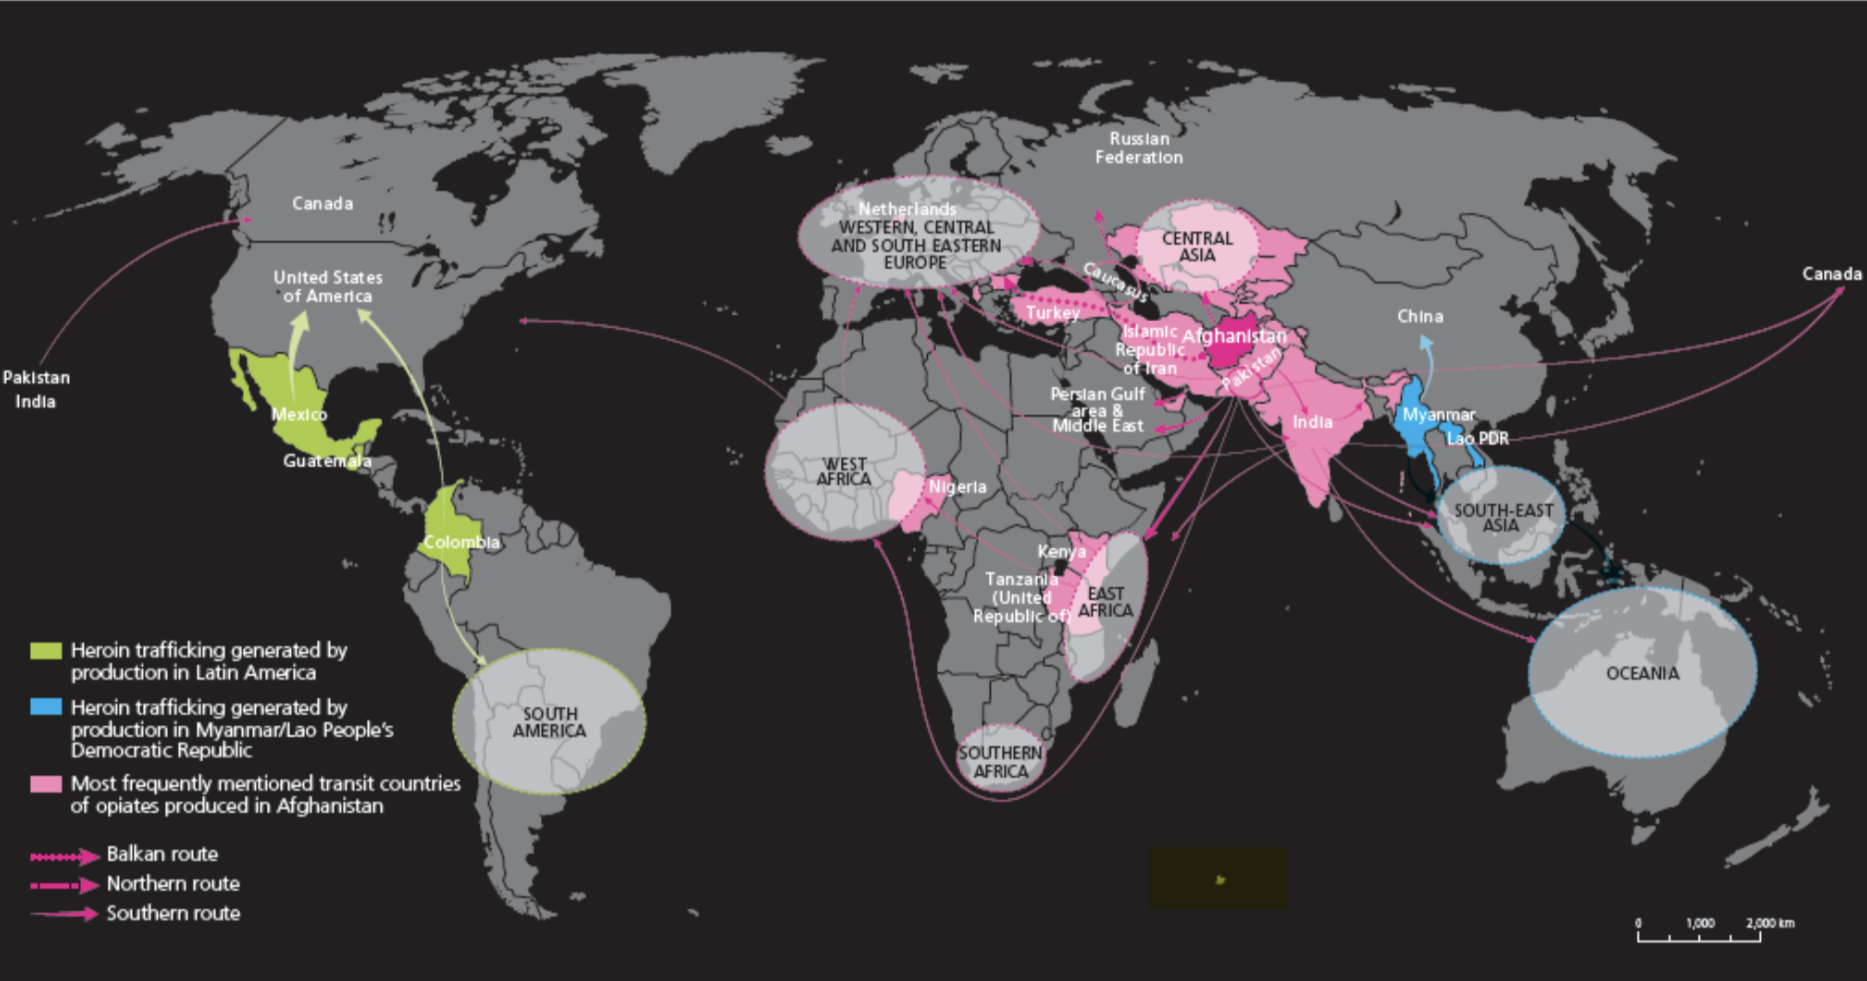
\includegraphics[width=17cm]{opiate_flows.png}
\normalsize\url{unodc.org/wdr2017/field/7.3.1_opiate_trafficking_flows.pdf}
\bigskip
\bigskip

\large\textbf{Cocaine}
\medskip

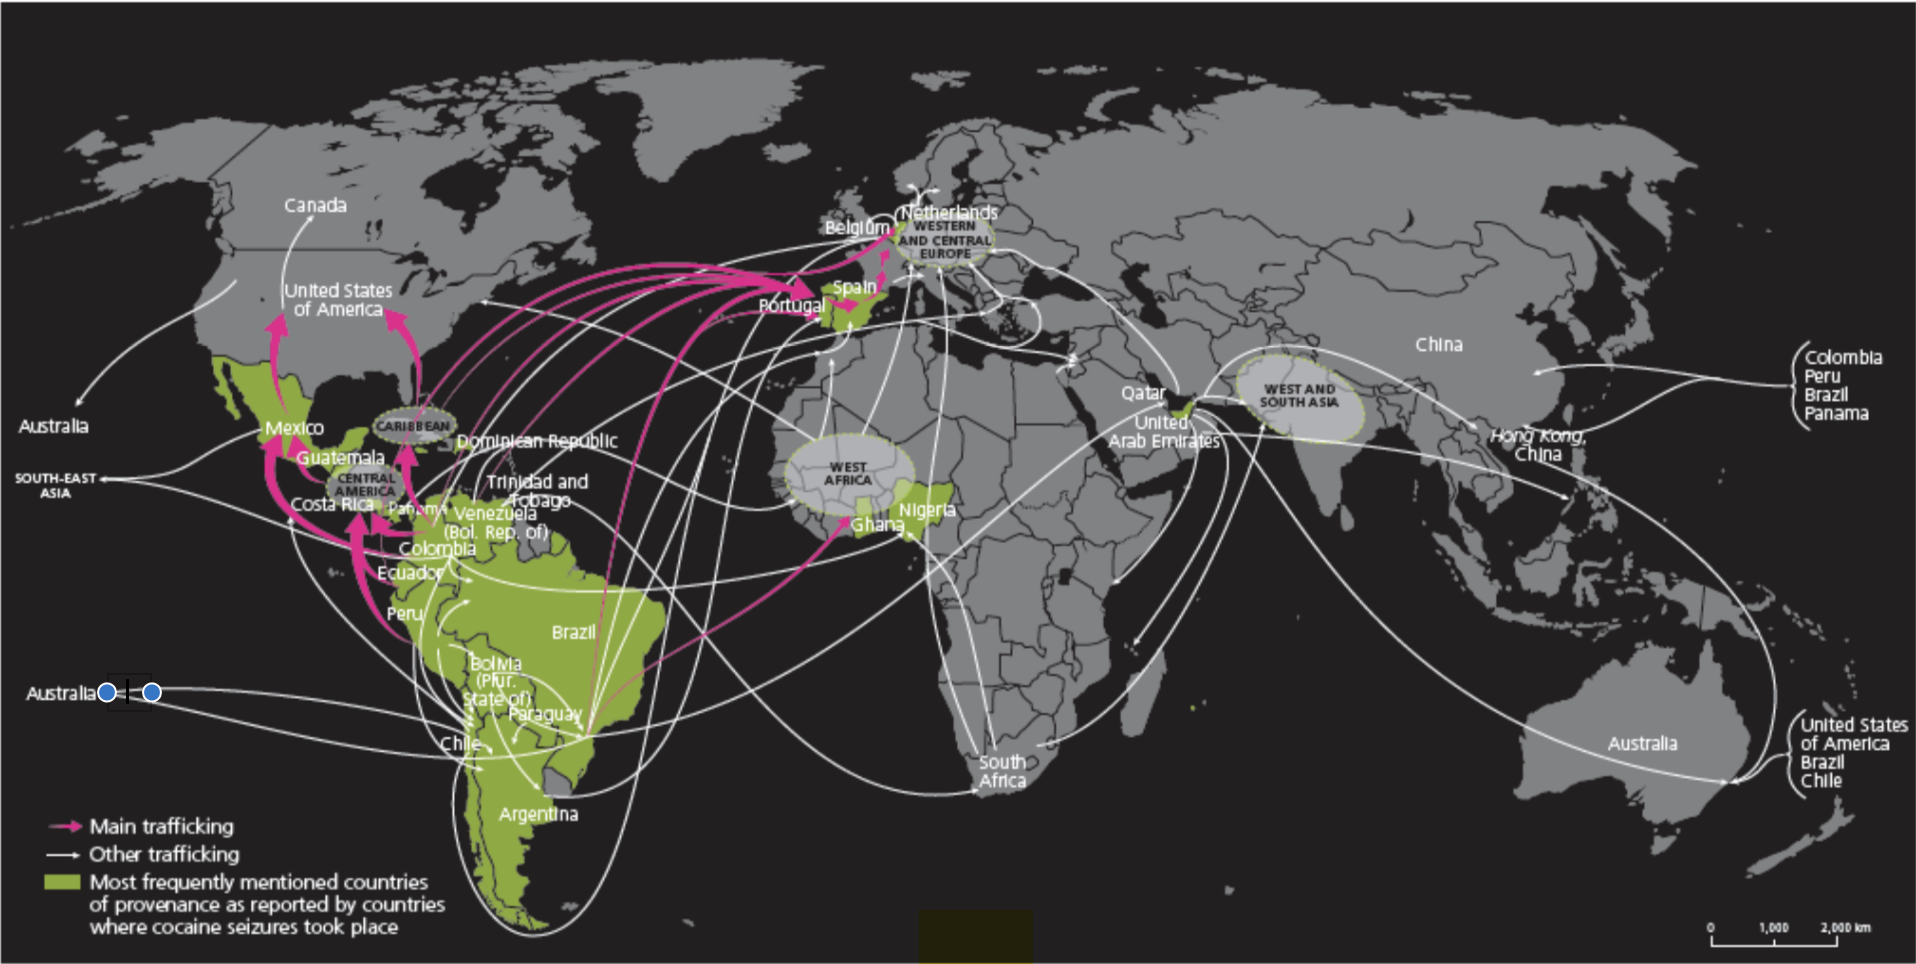
\includegraphics[width=17cm]{cocaine_flows.png}
\normalsize\url{unodc.org/wdr2017/field/7.3.2_cocaine_trafficking_flows.pdf}

\clearpage
\end{center}



\paragraph{Inefficiency} But despite incredible profits making their way back to the cartels, the drug business is incredibly inefficient. Of the \$100 billion Americans are spending annually, the Sinaloa Cartel (which has a 40 - 60\% share of the US market) only pulls in an estimated \$3 billion.\footnote{\url{nytimes.com/2012/06/17/magazine/how-a-mexican-drug-cartel-makes-its-billions.html}}
A closer look at annual drug seizures and wholesale/retail price differences shows the gross inefficiency of the traditional drug business model. In 2015, 7317 metric tons of cannabis and 864 metric tons of cocaine were seized (globally).\footnote{\url{unodc.org/wdr2017/field/Booklet_1_EXSUM.pdf}} Taking some liberties, if these drugs were able to be sold at United States ``street'' prices, additional revenue would come to $\sim$\$200 billion (and that doesn't even include seizures of heroin, methamphetamine, etc.).\footnote{Using prices from \url{rehabcenter.net/the-average-cost-of-illegal-drugs-on-the-street/}}
\\

For an enterprise with revenues rivaling Silicon Valley giants,\footnote{\url{justice.gov/sites/default/files/criminal-ocgs/legacy/2011/06/24/AAG Breuer Remarks_Mexican Drug Cartels_7.9.09.pdf}}
it would appear that the Sinaloa Cartel and its contemporaries in Columbia and Afghanistan have decidedly inefficient outcomes. This begins to explain the massive difference in price between street and wholesale drugs responsible for the greater than \$37 billion gap in American spending and market-share adjusted Sinaloa earnings.\footnote{(DoJ: Colombian and Mexican cartels reap \$18 billion to \$39 billion from drug sales in the United States each year - possibly biased) \url{nytimes.com/2012/06/17/magazine/how-a-mexican-drug-cartel-makes-its-billions.html}} % TODO bit of a run-on, rephrase.
Take, for example, the approximately 4900\% increase between Columbia and the United States that takes a kilogram of cocaine from \$2,000 to \$100,000 - and you can see that what someone pays for an illicit drug isn't for its inherent value. It is to compensate the combined risk to each part of the supply chain, for eluding the governments that tried to prevent it from getting to her.\footnote{\url{nytimes.com/2012/06/17/magazine/how-a-mexican-drug-cartel-makes-its-billions.html}}$^,$\footnote{\url{unodc.org/wdr2017/field/8.3_Price_and_Purity_Cocaine.xlsx}}
% TODO this is such a run-on. Fix it.


% from 2013 to 2015, darknet drug traffic grew 50% yoy unodc.org/wdr2017/field/Booklet_1_EXSUM.pdf

% percentages of drug trafficking offenses therecoveryvillage.com/drug-addiction/drug-trafficking-by-the-numbers/

% \paragraph{Examination of current state of technology in drug trade}?

% unodc.org/wdr2017/en/maps-and-graphs.html

% note - i will focus mainly on heroin and cocaine, since the illegal market for Marijuana will likely dwindle in the coming years as legalization rolls out in North America. 

%/ ==============================================================================================
%/ 									    	 ECONOMICS
%/ ==============================================================================================




%/ ==============================================================================================
%/ 									     DIGITAL DRUG TRADE
%/ ==============================================================================================
\section{Digital Drug Trade}

This glaring inefficiency clearly shows the incentive for innovation in the drug trade. Hundreds of billions of dollars of value are being tossed aside every year. It is this inefficiency (and the plethora of risks inherent to traditional illicit drug enterprise) that has given rise to a more decentralized model in online black markets.

\paragraph{Online Drug Trade} While it has only become generally recognized in recent years, the digital drug trade is as old as the internet itself. In fact, the world's first online transaction was a Stanford-MIT drug deal over the ARPANET.\footnote{\url{theguardian.com/science/2013/apr/19/online-high-net-drugs-deal}}$^,$\footnote{Maybe that's why they aren't in the Ivy League} The advent of Bitcoin as a semi-anonymous means of transacting online led to the creation of ``The Silk Road'' in 2011 - at the time the largest ever digital marketplace for illegal goods and services, especially drugs. Over the (approximately two-year) course of its existence, the Silk Road saw approximately \$200 million in transaction volume before being shut down.\footnote{\url{reuters.com/article/us-usa-bitcoin-trial-silkroad/u-s-sharply-reduces-silk-roads-estimated-sales-volume-idUSKBN0KP20N20150116}}
Unsurprisingly, a plurality of that volume (at least 30\%) came from the United States.\footnote{\url{en.wikipedia.org/wiki/Silk_Road_(marketplace)}}

\paragraph{Efficiency Improvements} Of note is the $\sim$\$12 million in commission the site's owners earned in that time - approximately 6\%.\footnote{ \url{en.wikipedia.org/wiki/Silk_Road_(marketplace)}} Compare this to the $\sim$90\% Sinaloa cartel loses to middlemen in the traditional drug economy (from above). This presents a strong incentive for entrepreneurs to form illicit markets, and for suppliers to participate. Furthermore, the weight moved by digital suppliers is relatively fractured - direct business-to-consumer transactions eliminate the necessity of the bulk shipments frequently seized by the state. It is not only more difficult for drug enforcement agencies to seize small shipments, but less rewarding and effective. In fact, many of these markets have instructions for suppliers on how to package goods so as to avoid detection.
\\

In addition, users do not have to worry about the possibility of violence that comes with an in-person drug deal. Reputation systems such as comments and reviews can give a good indication of the trustworthiness of a seller (not unlike Amazon) - again in contrast to ``sketchy'' meatspace transactions. All these factors contribute to the 50\% annual growth in the darknet drug economy.\footnote{\url{unodc.org/wdr2017/field/Booklet_1_EXSUM.pdf}}
\\

While the reactive intuition may be to see this as a problem, the case can be made that a modernization of the drug trade is a good thing. By eliminating street violence at the point of sale, it is possible we will see a reduction in user deaths by homicide. On a macro scale, the online drug trade also shows promise in reducing civilian casualties of the drug war - which have far outpaced those of the wars in Afghanistan and 
Iraq (including the ISIS era).\footnote{\url{pbs.org/wgbh/frontline/article/the-staggering-death-toll-of-mexicos-drug-war}}$^,$ \footnote{\url{en.wikipedia.org/wiki/Iraqi_Civil_War_(2014-present)}}


\begin{center}
\bigskip
\large{\textbf{Killings in Mexico v. Civilian Deaths in Afghanistan and Iraq (2007-2015)}}
\bigskip

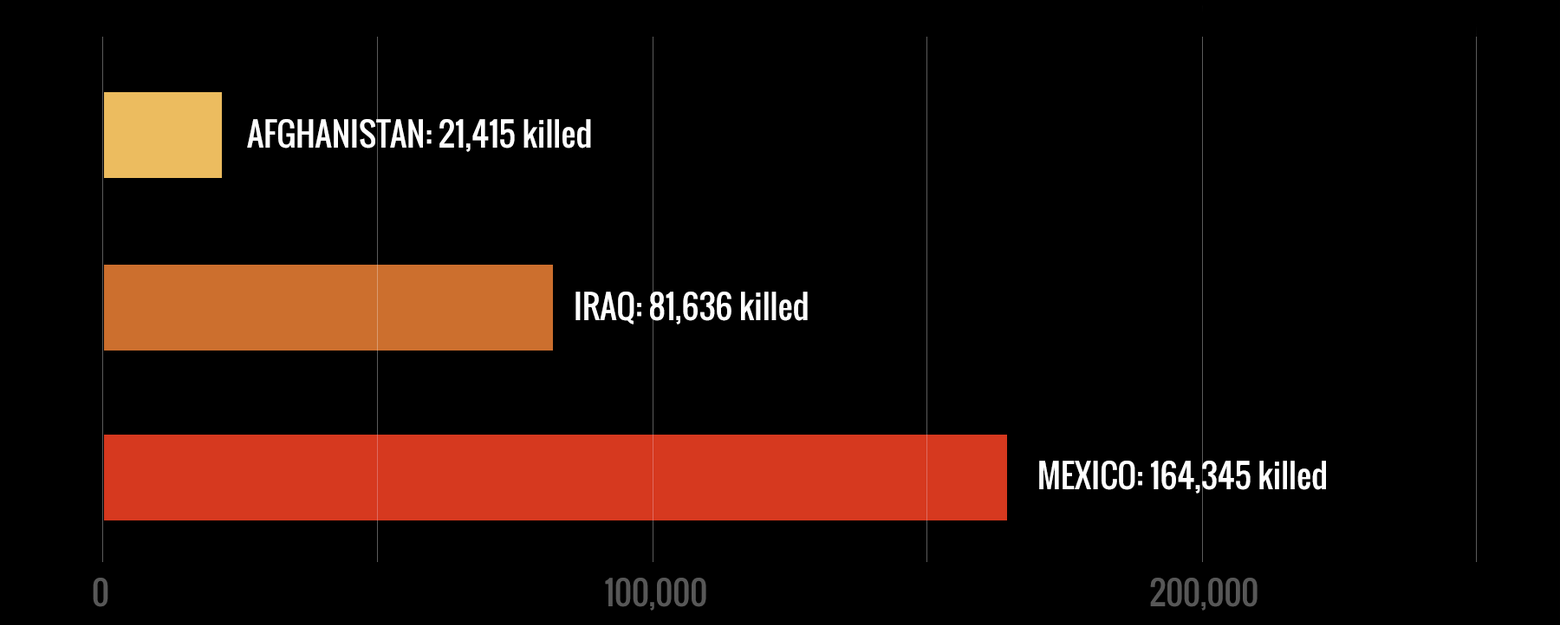
\includegraphics[width=12cm]{civilians.png}
\bigskip
\end{center}


\paragraph{Incarceration} Furthermore, the striking statistics on drug-related incarceration show an incredible opportunity for improved outcomes. Nearly 50\% of the United States federal prison population is incarcerated for drug-related crime.\footnote{\url{bop.gov/about/statistics/statistics_inmate_offenses.jsp}}  If advances in technology reduce the effectiveness of violence in the drug industry, and policing widespread small scale distribution proves implausible, we could see a major reduction in this number. Trying to remain objective, it is important to note that we cannot make any claims about the $\sim$18\% of prison inmates who committed their current offense for drug money.\footnote{\url{en.wikipedia.org/wiki/Drug-related_crime}} It is possible that number could rise as drug purchases become more convenient. However it is also possible that number will fall as substances become cheaper and the financial cost of addiction drops. The exciting thing is that we will find out - since there is nothing that can/will be done to stop the growth of online black markets.
\\

It is possible we will reach some kind of equilibrium - ``hard'' drugs will likely not become legal for tens of years, yet there is little chance demand will halt. A reasonable ceasefire may persist if the drug trade becomes less violent and small-time dealers find safety in their numbers. The government gets to say that drugs are illegal without the consequences of enforcement, suppliers get their profits without seizures or risk of violence from the competition, and users get the substances they want delivered to the safety of their doorsteps. In short, hopefully everyone can just ``chill out.''\footnote{And we can direct law enforcement funding to addiction treatment and rehabilitation}


%/ ==============================================================================================
%/ 									     DIGITAL DRUG TRADE
%/ ==============================================================================================




%/ ==============================================================================================
%/ 									     	  XMR
%/ ==============================================================================================
\section{XMR}

The technology that will enable these developments is the Anonymous Blockchain. While Bitcoin's public chain is the big brand in the cryptocurrency space, the limitations of the legacy technology quickly led to more advanced financial systems. While its code is host to many other deficiencies, in this case Bitcoin's public blockchain was an incredible disadvantage for users seeking financial anonymity. This market incentive for privacy has fueled the rise of Monero (XMR) - today's most popular Anonymous Blockchain.
\\

Skipping over 
(but linking)\footnote{\url{themerkle.com/the-early-history-of-monero-in-500-words/}} the crypto-political story of XMR's origin, we can get directly into the present state of the tech.
Hopefully, the pages above have shown the plethora of incentives for financial privacy inherent to illegal markets. Indeed, the past few years have seen Monero undergo the familiar meteoric cryptocurrency ascent in price and volume. Unlike many others, however, XMR is already thoroughly useful. While the Silk Road and Silk Road 2.0 did not support the currency, the late AlphaBay began accepting Monero on September 1st, 2016.\footnote{\url{deepdotweb.com/2016/08/23/alphabay-oasis-markets-begin-accepting-monero-payments/}} XMR volume and price immediately spiked, which should give a good intuition for user need and market perception of the online drug market.\footnote{\url{coinmarketcap.com/currencies/monero/#charts}}
\\
% TODO
	% these are like the Pablo Escobar stories of CyberNarcos/NarcoTechnicals


	% DEA unknown amount of XMR seizure
	% 30\% of all offenses in 2013 were related to drug trafficking
	% therecoveryvillage.com/drug-addiction/drug-trafficking-by-the-numbers/



So how does the technology behind Monero work under the hood? The answer reveals a beautiful (though complex) system. Unfortunately I will have to assume familiarity with the basics of blockchain technology, or this section would run several pages longer. I will also skip over some of the cool innovations in XMR that are not essential to its mathematical privacy, since this paper is about financial anonymity.\footnote{Dynamic block sizing, send vs. view keys, power of ten mixing, memory-heavy mining/the CryptoNight algorithm, and more.}

\paragraph{Cryptography Basics} Digital Signature Algorithms and public-private key cryptography are some of the coolest bits of number theory ever created.\footnote{\url{en.wikipedia.org/wiki/Elliptic_Curve_Digital_Signature_Algorithm}} Unfortunately, current signature algorithms will likely fall to quantum computers - at which point they will hopefully be replaced with extreme 
prejudice.\footnote{\url{eprint.iacr.org/2015/1018.pdf}} Until then, however, they remain one of the most useful innovations in human 
history.\footnote{\url{en.wikipedia.org/wiki/Post-quantum_cryptography}}
The inner workings of the ECSDA cryptography underneath the Monero blockchain are beyond the scope of this paper.\footnote{Mainly because I brushed up on RSA and had a good explanation and example ready to go before realizing Monero doesn't use RSA.} However, that should not preclude the reader from a basic understanding of the genius behind public/private key cryptography. The classic encryption problem goes back to Roman times - how can you get a secret message to someone without a shared secret? For example, Caesar's cipher (where ``abc'' becomes ``bcd'' with secret key 1) is trivially breakable. Furthermore, the recipient of a message must already know the secret key in this system, which defeats the whole purpose - because the secret key must have been sent in an unencrypted message.

\paragraph{Public/Private-key Cryptography} For an intuition of public/private-key crypto, you can imagine that your friend (let's call him Ross) wants to send you a box full of valuables, and receive payment for said valuables. You both have the ability to make keys and locks. Any key or lock he sends you may be intercepted and duplicated. How can you send/receive items without possibility of theft? Well, Ross can create one lock and a corresponding key. He keeps the key secret, but publishes the design of the lock so everyone can make a copy if they like (so they can only lock, not unlock). You do the same, so now Ross has a copy of your lock and you have a copy of his. He locks the box with your lock and sends it to you. Nobody can unlock the box but you, since you have the secret key. After opening the box and removing the contents, you can now put some cash in there for Ross, use his public lock to seal the box, and send it back safely.

\paragraph{Transactions} In this analogy, ECSDA is the process of creating a lock and key. The lock is the public key that anyone can use to encrypt a message (or amount of money) they want to send your way. And of course the key is the private key. Now in a public blockchain like Bitcoin, sending transactions works in a similar way. One of the cool things about public/private key cryptography is that you can ``lock'' things with your private key, too. This means that Ross can broadcast a message that was locked with his private key, and only his public key can decrypt it. Therefore, since we all have his public key, we can verify that it was in fact Ross who wrote the message. So if I want to pay Ross in Bitcoin, I can broadcast a message to the network declaring that ``I send Ross one BTC.'' If I also lock that message with my private key and publish it, everyone can decrypt with my public key and only my public key, and double check that it isn't someone trying to misappropriate my funds. 

\paragraph{UTXOs} The sneaky ones among you might think ``\emph{I could just say that I send 20 BTC, even if I only have a couple.}'' Note that in Bitcoin your ``address'' is a hash of your public key. So instead of saying ``\emph{I send Ross one BTC},'' we publish something 
more like ``\texttt{128uafspd} \emph{sends} \texttt{2p090asfd} \emph{one BTC}.'' This is where Unspent Transaction Outputs (UTXOs) come in. UTXOs are the sum of transactions that have been verified and sent your way, tracing all the way back to when they were mined. So on the Bitcoin blockchain, your balance is effectively the number of UTXOs tied to your public key for which you can produce a valid signature. 

\clearpage

\paragraph{Private Transactions} Now if you are buying/selling drugs, this is a pretty scary concept - everyone can see that you did something illegal or that your gains are ``ill-gotten.'' But without these naked financials, how can people verify your transactions and wealth (UTXOs)? The solution comes from a beautiful concept called a 
``Ring Signature.''\footnote{\url{en.wikipedia.org/wiki/Ring_signature}}$^,$\footnote{\url{https://link.springer.com/content/pdf/10.1007/3-540-45682-1_32.pdf}} Originally designed for whistleblowers, a ring signature is a way for someone to sign and send a message without revealing his identity. Remember, our original implementation above requires that verifiers know the sender's identity so they can check using the right public key.

\paragraph{Ring Signatures} In a ring signature, you gather several other people's public keys, and use them to lock your message. This is where it's important to note a small difference from the intuition of ``locks'' and ``keys.'' You can use a cryptographic key as a metaphorical lock \emph{and} as a metaphorical key. In the case of the ring signature algorithm, you create one big lock from several public keys and your own private key. Like the ECSDA algorithm, the exact process through which this is done is beyond the scope of this paper. On a basic level though, encryption works by recursively XOR chaining a traditional/symmetric-key algorithm (like Caesar, for example). This is trivial to decrypt if you know who was in the ring - at which point you have verified that the message originated from \emph{someone} in that group.

\paragraph{Unlinkable Payments} The previous paragraph gave the basics of how a sender can remain anonymous, but what about the recipient? Whereas in Bitcoin we redirected UTXOs to their new owners by signing over directly to their public key, with XMR this would expose the beneficiary's identity. The Monero protocol gets around this in a clever way. Instead of having public keys be tied explicitly to received transactions, the protocol wraps up transaction outputs in an indirect way such that only the private key holder could even know he was the recipient of the transaction. So by constantly scanning the blockchain and looking for transactions I can decrypt, I become the only person that knows when I have received funds, and how much wealth (UTXOs) I have to my name.%\footnote{Note: I had hoped to dive much deeper into the advanced mathematics of Monero, however over the course of this project I realized it would take several weeks (if not months) to fully understand the technology. There is so much more to learn, which unfortunately makes this section a massive oversimplification of the core concepts.}
\\

While there are textbooks worth of mathematics behind these and the other concepts that form the Monero system, hopefully this section gives a basic understanding of the state of the art. This is a technology that will be around for a long time, regardless of regulatory oversight. For this reason, it is important to be informed and continue to stay up to date with its implementation and use as volume continues to grow.


\clearpage
%/ ==============================================================================================
%/ 									     	  XMR
%/ ==============================================================================================




%/ ==============================================================================================
%/ 									       CONCLUSION
%/ ==============================================================================================
\section{Conclusion}

In our discussion, we first touched on the current state of the drug trade: thriving, yet inefficient. We saw the damage caused by America's drug war, and the futility of law enforcement efforts to prevent the illegal drug trade. As long as the status quo persists, both the government and the cartels will go on killing and incarcerating hundreds of thousands of civilians and citizens. But the ``Insatiable North American Nose''\footnote{\url{nytimes.com/2012/06/17/magazine/how-a-mexican-drug-cartel-makes-its-billions.html}} is not without blame. Our nation's indiscriminate purchase of conflict-zone drugs is the market force underlying all this chaos.
\\

Despite the inevitability of demand however, there is hope for a more peaceful equilibrium. Like the nerds behind ``MoneyBall,'' it may be that cryptographers and mathematicians become the Tech-Narcos of the 21st century. It is my hope that the advent of financial privacy and explosion of darknet drug trade will dramatically reduce the casualties of the drug war, and the technological sophistication of XMR will leave Governments and Cartels alike helpless to stop it.
I remain optimistic that the creators of the next big free market will introduce civilization to an historically uncivilized industry,\footnote{Learning from the mistakes of the Dread Pirate Roberts} and the next generation of the illicit drug trade will look more like \emph{Silicon Valley} and less like \emph{Scarface}. 


\clearpage


% We touched on the state of the drug trade
% These markets exist because of demand
% There's nothing we can do to stop it, best approach is to try to save lives
% This is where a more civilized drug trade on the dark net comes in
% Monero is the tech to do it. Useful for other things as well, it's a great technology. But this is a clear cut use case.

% hope we can all chill out and stop killing each other, so we can have more Silicon Valley and less Scarface.

%/ ==============================================================================================
%/ 									       CONCLUSION
%/ ==============================================================================================









%/ ==============================================================================================
%/ 									       References
%/ ==============================================================================================
\pagebreak
\section{Miscellaneous References}
\footnotesize

\url{nytimes.com/2012/06/17/magazine/how-a-mexican-drug-cartel-makes-its-billions.html}\\

\url{history.com/news/10-things-you-should-know-about-prohibition}\\

\url{en.wikipedia.org/wiki/Ring_signature}\\

\url{people.xiph.org/~greg/confidential_values.txt}\\

\url{arstechnica.com/information-technology/2013/10/a-relatively-easy-to-understand-primer-on-elliptic-curve-cryptography/}\\

\url{en.wikipedia.org/wiki/Illegal_drug_trade#History}\\

\url{unodc.org/unodc/en/drug-trafficking/index.html}\\

\url{en.wikipedia.org/wiki/Illegal_drug_trade_in_the_United_States}\\

\url{obamawhitehouse.archives.gov/sites/default/files/ondcp/policy-and-research/wausid_results_report.pdf}\\

\url{wired.com/2015/04/silk-road-1/}\\

Thomas H. Cormen, Clifford Stein, Ronald L. Rivest, and Charles E. Leiserson. 2001. Introduction to Algorithms (2nd ed.). McGraw-Hill Higher Education. \\

\url{developer.com/java/ent/article.php/3092771/How-Digital-Signatures-Work-Digitally-Signing-Messages.htm} \\

\url{bitcoin.com/info/how-bitcoin-transactions-work}\\

\url{people.xiph.org/~greg/confidential_values.txt}\\

\url{en.wikipedia.org/wiki/Symmetric-key_algorithm}\\

\url{lab.getmonero.org/pubs/MRL-0005.pdf}\\

\url{github.com/monero-project/research-lab/blob/master/whitepaper/whitepaper.pdf}\\

%/ ==============================================================================================
%/ 									       References
%/ ==============================================================================================

\end{document}
















